\section{Q18: no fixed depth, history, or delay is universally sufficient}
\label{sec:q18}

\textbf{There is no single view that is enough for every decision.} Q18 tests the vendor's
implicit promise most directly: that a deeper, longer, fresher feed is uniformly better,
so a buyer can pick one sufficient configuration and stop paying for more. We cross book
depth (one versus five levels), history (instantaneous versus a longer window), and update
delay (current versus delayed) and fit every cell with three model families on $18$
sampled-L2 contracts over $9$ BTC/ETH dates, for $120$ fits.

\paragraph{The effect has no common sign.} Figure~\ref{fig:q18} shows the relative-loss
gap of the full depth-plus-history view against the reduced view for every
model$\times$asset$\times$factor cell on the transfer dates. A universal sufficiency
threshold would make these gaps line up on one side of zero. They do not. Adding depth
helps BTC logistic regression ($+0.077$ relative loss) but hurts the BTC perceptron with a
delayed view ($-0.049$). Adding depth helps ETH logistic regression ($+0.104$) while
removing history barely moves ETH gradient boosting. The signs flip with model and with
asset, and many simultaneous day-clustered intervals straddle zero, so the panel cannot
reject ``no effect'' for a fixed rule. A separate optimizer diagnostic sharpens the
disagreement: shallow inputs fit BTC better while deeper inputs fit ETH better, at both
$60$ and $600$ iterations, so the two assets ask for opposite feeds.

\begin{figure}[t]
\centering
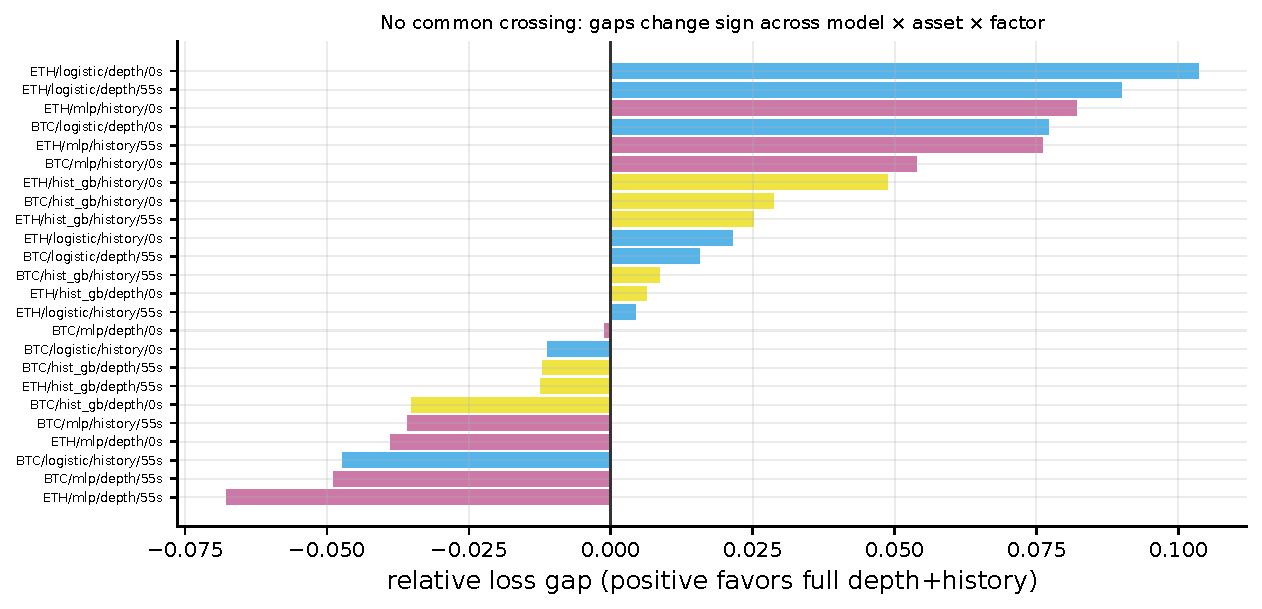
\includegraphics[width=\linewidth]{figures/fig_q18_no_crossing.pdf}
\caption{\textbf{Q18: no common crossing.} Relative-loss gap (full depth+history minus
reduced view. Positive favors the richer view) for every model$\times$asset$\times$factor
$\times$delay cell on the transfer dates, sorted. A universal sufficiency threshold would
put all bars on one side of zero. Instead the effect changes sign across configurations,
and its magnitude is small relative to the spread.}
\label{fig:q18}
\end{figure}

\paragraph{What the negative does and does not say.} It does not say depth is useless.
Some cells genuinely improve with more information, and the certified reading in a stricter
companion analysis (six asset--model combinations, both assets, at least two families
required) certifies a clock-induced change in $0$ of $6$ cases while explicitly refusing to
convert a failure-to-certify-noninferiority into a proof of insufficiency. What the panel
rejects is the \emph{simple} rule, ``five levels are always enough'' or ``freshness
always makes depth valuable'', that a one-size feed decision would need. Extra market
detail behaves like adding sensors to a control system: the sensors may carry information,
but a particular learner, sample, or timing alignment can fail to exploit it, and here the
exploitation fails inconsistently across exactly the axes a buyer would want to hold fixed.

\paragraph{Relation to representation-sufficiency theory.} Formal work defines
decision-sufficient representations as those that preserve the optimal action
\citep{ye2026learning, walsh2026support}, and depth-aware forecasting studies map
predictive value to book levels \citep{briola2024hlob, briola2024deep}. Our panel is the
empirical complement: a classifier plateau cannot estimate a theoretical sufficient
dimension, but it can show that no fixed observable configuration is sufficient across
assets and models on real data. The sufficiency question is therefore conditional by
nature, and a leaderboard that reports one average curve hides the sign changes that
decide whether a feed is worth buying.
